% This is LLNCS.DEM the demonstration file of
% the LaTeX macro package from Springer-Verlag
% for Lecture Notes in Computer Science,
% version 2.4 for LaTeX2e as of 16. April 2010
%
\documentclass{llncs}
%
%\usepackage{makeidx}  % allows for indexgeneration
\usepackage{graphicx}
	\graphicspath{{images/}} 
%\usepackage{cite}
\usepackage[linesnumbered,ruled]{algorithm2e}
\usepackage{courier}
\usepackage{hyperref}
    \hypersetup{colorlinks=true,allcolors=blue}
\usepackage{listings}
	\lstset{
  		basicstyle=\ttfamily,
  		frame=none, 
  		breaklines=true,
  		numbers=left,
  		xleftmargin=2.5em,
  		framexleftmargin=0em,
    	emphstyle=\textbf,
    	float=t
	}
	\lstdefinestyle{ocl}{
  		emph={
        	context, inv
    	}
	}
	\lstdefinestyle{cbp}{
	    basicstyle=\ttfamily\scriptsize,
  		emph={
        	session, create, of, type,
        	set, to, add, hire
    	}
	}
	\lstdefinestyle{xmi}{
		basicstyle=\ttfamily\scriptsize,
  		emph={
        	Node, children
    	}
	}
	\lstdefinestyle{xml}{
	    basicstyle=\ttfamily\scriptsize,
  		emph={
        	register, create, add, to, resource,
        	from, eattribute, remove, ereference,
        	set, unset, session, Roy, Jen,
        	Moss, Richmond
    	}
	}
	\lstdefinestyle{java}{
	    basicstyle=\ttfamily\scriptsize,
  		emph={
        	case, UNSET,
        	instanceof, else, if, void,
        	new, UnsetEAttributeEvent,
        	UnsetEReferenceEvent,
        	@override, public, class, extends
    	}
	}
	\lstdefinestyle{eol}{
	    basicstyle=\ttfamily\scriptsize,
  		emph={
        	var, new, for, in, create, set, of, with, 
        	unset, to, add, remove, delete, register,
        	from, position, from, move-within, session, \.
    	}
	}

\begin{document}
\renewcommand{\thelstlisting}{\arabic{lstlisting}}
\renewcommand{\labelitemi}{$\bullet$}
\newcommand{\dk}[1]{\textbf{[DK: #1]}}

\title{Change-based Persistence and Its Loading Optimisation}
%
\titlerunning{Change-based Persistence and Its Loading Optimisation}  % abbreviated title (for running head)
%                                     also used for the TOC unless
%                                     \toctitle is used
%
\author{Alfa Yohannis \and Dimitris Kolovos \and Fiona Polack }
%
\authorrunning{Alfa Yohannis et al.} % abbreviated author list (for running head)
%
%%%% list of authors for the TOC (use if author list has to be modified)
%\tocauthor{Dimitris Kolovos, Fiona Polack, Alfa Yohannis}
%
\institute{Department of Computer Science, University of York, United Kingdom\\
\email{\{ary506, dimitris.kolovos, fiona.polack\}@york.ac.uk}}

\maketitle              % typeset the title of the contribution

\begin{abstract}
In this paper, we propose a change-based approach for persisting models conforming to object-oriented (MOF/Ecore) metamodelling architectures. We demonstrate how change-based persistence enables high-performance incremental model processing (e.g. transformation, validation) by reducing the cost of identifying fine-grained changes in evolving models. We illustrate a language-independent change-based model representation format and an optimised model loading algorithm that seeks to avoid replaying changes that have no impact on the eventual state of the model. We report on benchmarks that compare model loading and saving performance of the proposed change-based representation against the standard state-based representation format (XMI). Our results show considerable savings in terms of persisting and identifying changes made to models at an increased -- but linear -- model loading cost.
\end{abstract}

\section{Introduction}
\label{sec:introduction}
To reap the benefits of Model-Based Software Engineering in the context of complex and large systems, the ability to process large models in an incremental fashion as they evolve is essential. Existing incremental model processing techniques only yield limited performance benefits due to imprecise and slow model change detection capabilities or are only limited to a single-developer environment, which is not applicable for real-world software development projects.


Instead of persisting snapshots of states of models, we propose turning models inside out and persisting their change history. The proposed approach has the potential to deliver step-change performance benefits in incremental model processing, as well as a wide range of other benefits and novel capabilities. While persisting changes to large models is expected to be much faster and resource-efficient compared to state-based approaches, loading models into memory by naively replaying the entire change history is expected to have a significant overhead. To address this challenge, we propose algorithms and data structures that will reduce the cost of change-based model loading (e.g. by recording and ignoring events -- events that are later overridden or cancelled out by other events), extending the preliminary work of Yohannis et al. \cite{yohannis2017turning}.

The rest of the paper is structured as follows. Section \ref{sec:change_based_persistence} presents briefly the concept of change-based persistence. Section \ref{sec:related_work} provides an overview of existing related work. Section \ref{sec:proposed_approach} overviews our proposed approach. The algorithms to optimise the loading time of change-based persistence, as well as the CBP's performance evaluation, are presented in Sect. \ref{sec:loading_time_optimisation} and Sect. \ref{sec:performance_evaluation} respectively. 
Section \ref{sec:limitations} presents the limitation of our approach and Sect. \ref{sec:conclusions} concludes this paper.

\section{Change-based Persistence}
\label{sec:change_based_persistence}
A change-based model or change-based persistence (CBP) is a concept of model that records incremental changes -- incrementality -- of a model and uses the records for a variety of purposes, such as model analytics, optimising execution of model operations (e.g. validation, transformation), or generating different versions of a model based on its timeline. The incremental changes can be presented as, but not limited to, a collection of events arises from operations applied to a model during its construction. 

\begin{figure}[ht]
\begin{minipage}[t]{0.39\linewidth}
    \centering
    \raisebox{0.75\height}{
    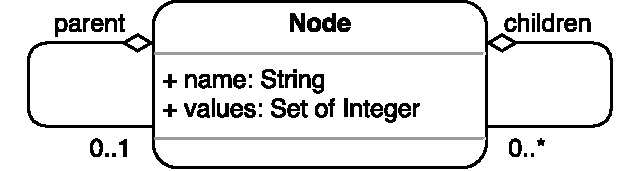
\includegraphics[width=\linewidth]{node_metamodel}}
    \caption{A class diagram of a simple tree modelling language.}
    \label{fig:node_metamodel}
\end{minipage}
    \hfill
\begin{minipage}[t]{0.59\linewidth}
    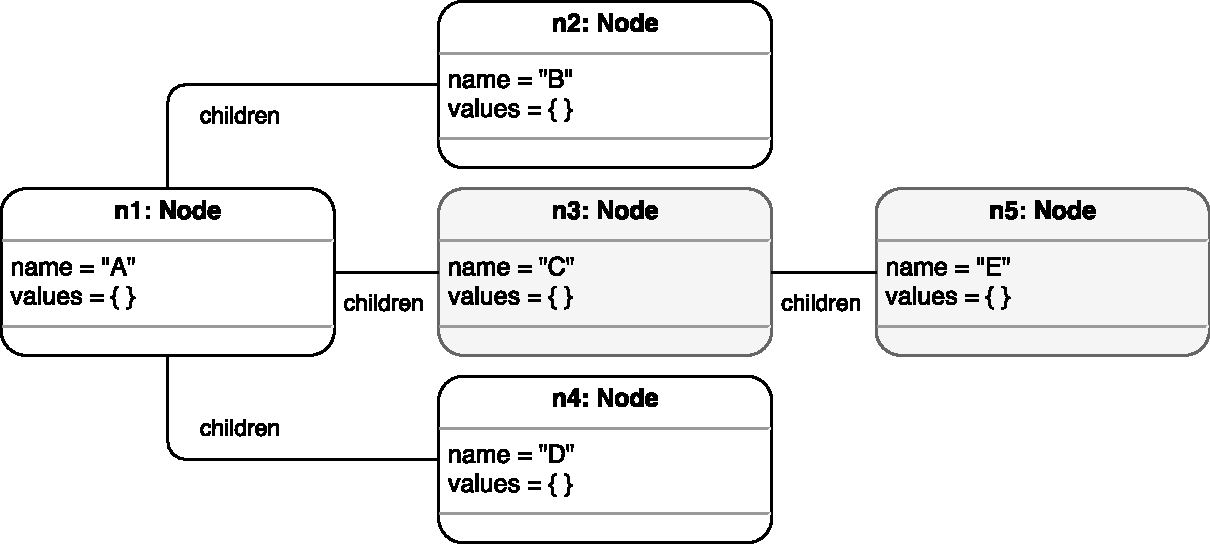
\includegraphics[width=\linewidth]{initial_chart}
    \caption{A tree model with 5 nodes. Node \emph{n3} and \emph{n5} are deleted from a model.}
    \label{fig:initial_model}
\end{minipage} 
\end{figure}

To help us explain the concept of incrementality and our approach to optimise its loading time, we use a simple tree modelling language (Fig. \ref{fig:node_metamodel} shows its class diagram) to create examples of  tree models to support our explanation. Essentially, the model consists of nodes in which every node can have one to many, containment references\footnote{Containment reference is a composite relationship which an object holds a reference to another object. Deleting the former deletes the the latter as well.} with other nodes (\emph{children} relationship). A node can can also have a have a single containment reference, \emph{associate} relationship, with another node. Every node has two attributes, \emph{name} and {values}. Attribute \emph{name} is a type of String and attribute \emph{values} contains a set of Integer.

As the first, main example for this paper, we create a tree model as shown in Fig. \ref{fig:initial_model} using the modelling language in Fig. \ref{fig:node_metamodel}. Initially, the model consists of five nodes \emph{n1}, \emph{n2}, \emph{n3}, \emph{n4}, and \emph{n5}. Node \emph{n1} contains three direct nodes \emph{n2}, \emph{n3}, and \emph{n4}, and node \emph{n3} contains node {n5}. Later, nodes \emph{n3} are deleted from the model, which means node \emph{n5} is also deleted since node \emph{n5} is contained by node \emph{e3} (deleted nodes are coded with grey colour). After every modification of the model, the model needs to be (1) validated against a domain-specific constraint (a node can only have 3 or less children), and (2) transformed into a number of HTML files through a model-to-text transformation. Each file contains the name of the node, and the names of its direct children.

Before nodes \emph{n3} and \emph{n5} are deleted from the model, when the validation constraint is evaluated against the initial model (Fig. \ref{fig:initial_model}), it verifies that each of the five nodes has three or less children, and the model-to-text transformation then produces five HTML files that correspond to the nodes in the model. The model is then updated by deleting nodes \emph{n3} and \emph{n5} from the model, which also node remove node \emph{n3} from node \emph{n1}. 

A non-incremental model validation engine, after the removal of nodes \emph{n3} and \emph{n5}, would treat the model of Fig. \ref{fig:initial_model} as a new model and will evaluate the constraint above against every node in the model. An incremental model validation engine, on the other hand, would identify that the previously established satisfaction of the constraint for nodes \emph{n2} and \emph{n4} are not affected by the changes made, and would only re-evaluate the constraint for nodes \emph{n1} instead. 

Similarly, a non-incremental model-to-text transformation would generate and overwrite all output text files from scratch. On the contrary, an incremental model-to-text transformation, would identify that it only needs to delete the HTML files of nodes \emph{n3} and \emph{n5} since they have been removed and generate a new HTML file for node \emph{n1} as the number of its children has changed -- but not the text files of nodes \emph{n2} and \emph{n4}, as these cannot have been affected by the changes made to the model.

While the overhead of executing transformations and validation constraints on small models like the one in Fig. \ref{fig:initial_model} is not significant, non-incremental execution can become a significant bottleneck for large evolving models, especially when a development cycle is closer to its end, when developers tend to perform many small changes to fine-tune systems. Thus, a sophisticated impact analysis is needed to reduce the amount of code regeneration in order to keep the overhead minimum \cite{selic2003pragmatics}.  

%As an example to explain incremental re-execution of queries on structured models, we use an OCL implementation of the domain-specific constraint in List. \ref{lst:constraint}.
%
%\begin{lstlisting}[style=ocl,caption={OCL constraint requiring that nodes directly can only have 3 children or less.},label=lst:constraint]
%context Node
%inv equalOrLessThan3: self.children->size() <= 3
%\end{lstlisting}
%
%During the initial evaluation of the constraint on the model of Fig. \ref{fig:initial_model} (before the removal of nodes \emph{n3} and \emph{n5}), an incremental OCL engine would compute the property access trace displayed in Table \ref{tab:property_access_trace} as a side-product. Now, when the model is updated (after the removal of nodes \emph{n3} and \emph{n5}), the execution engine can identify that: (1) There are two elements, \emph{n3} and nodes \emph{n5}, have been removed from the model for which the constraint has been evaluated; (2) The value of the children property of node \emph{n3} has changed, and as such, it needs to re-evaluate the constraint on this model-element.
%
%\begin{table}[ht]
%\centering
%\caption{Property-access trace of the evaluation of the constraint in List. \ref{lst:constraint} on the model of Fig. \ref{fig:initial_model}.}
%\begin{tabular}{p{3cm} p{1.5cm} p{1.5cm} p{1.5cm}}
%\hline 
%\textbf{Constraint} & \textbf{Context} & \textbf{Accessed Element} & \textbf{Accessed Property} \\ 
%\hline 
%\emph{Node.equalOrLessThan3}  & \emph{n1} & \emph{n1} & \emph{children} \\ 
%\emph{Node.equalOrLessThan3}  & \emph{n2} & \emph{n2} & \emph{children} \\ 
%\emph{Node.equalOrLessThan3}  & \emph{n3} & \emph{n3} & \emph{children} \\ 
%\emph{Node.equalOrLessThan3}  & \emph{n4} & \emph{n4} & \emph{children} \\ 
%\emph{Node.equalOrLessThan3}  & \emph{n5} & \emph{n5} & \emph{children} \\ 
%\hline 
%\end{tabular} 
%\label{tab:property_access_trace}
%\end{table}

\section{Related Work}
\label{sec:related_work}
There has been some work related to change-based persistence. In the pioneering work of Egyed \cite{egyed2011automatically}, in order to achieve incremental re-execution of (deterministic) queries on structured models, an execution engine needs to (1) record model element property accesses during the initial execution of the queries, (2) identify new and deleted elements and modified model element properties in the new version of the model, and (3) combine the information collected in the steps one and two to identify the subset of (potentially) affected rules/queries/templates that need to be re-executed. Egyed has shown that the property-access recording approach is applicable to queries of arbitrary complexity, as long as they are deterministic. More recent work has shown that variants of this approach can be used to achieve incrementality in a wide range of model processing operations, including model-to-model transformation \cite{jouault2010towards}, model-to-text transformation \cite{ogunyomi2015property}, model validation, and pattern matching \cite{rath2012derived}---as long as changes to models can be precisely identified (step 2 above).

There are two approaches in the literature for identifying changes in models in order to enable incremental re-execution of model processing operations, emph{model differencing} and \emph{notifications}. \emph{Model differencing} approach eliminates the coupling between modelling tools and incremental execution engines. Instead of depending on live notifications, in this approach the developer in charge of automated model processing, needs to have access to a copy of the last version of the model that the model processing program (e.g. the model-to-text transformation) was executed upon, so that it can be compared against the current version of the model (e.g. using a model-differencing framework such as SiDiff \cite{kelter2005generic} or EMFCompare\footnote{\url{https://www.eclipse.org/emf/compare/}}) and the delta can be computed on demand. The main advantage of this approach is that it works well in a collaborative development environment where typically developers have distinct roles and responsibilities. On the downside, model comparison and differencing are computationally expensive and memory-greedy (both versions of the model need to be loaded into memory before they can be compared), thus largely undermining the time and resource saving potentials of incremental re-execution. This approach is adopted by the Xpand model-to-text transformation language. According to the developers of the language, using this approach, a speed-up of only around 50\% is observed compared to non-incremental transformation\footnote{\url{http://wiki.eclipse.org/Xpand/New_And_Noteworthy\#Incremental_Generation}}, which is consistent with our experience from using Xpand.

In \emph{notification} approach, the incremental execution engine needs to hook into the notification facilities provided by the modelling tool through which the developer edits the model, so that the engine can directly receive notifications as soon as changes happen (e.g. a node (\emph{n5}) has been deleted, the name property of node \emph{n5} has been changed to ``E"). This is an approach taken by the IncQuery incremental pattern matching framework \cite{rath2012derived} and the ReactiveATL incremental model-to-model transformation engine \cite{ogunyomi2015property}. The main advantage of this approach is that precise and fine-grained change notifications are provided for free by the modelling tool (and thus do not need to be computed by the execution engine---which as discussed below can be expensive and inefficient). On the downside, this approach is a poor fit for collaborative development settings where modelling and automated model processing activities are performed by different members of the team.

In summary, incremental model processing currently delivers significant performance benefits only in a single-developer environment where the modeller is also responsible for performing all the (incremental) model processing operations. As a result, in collaborative development environments, developers need to either forgo incremental model processing altogether or to work around this limitation by manually steering model processing programs to process only subsets of their models, which is cumbersome and error prone.

\section{Proposed Approach}
\label{sec:proposed_approach}
The ambition of this research is to enable high-performance incremental model management in collaborative software development environments by challenging one of the fundamental assumptions of contemporary modelling frameworks and tools: as opposed to persisting snapshots of the state of models (which is what virtually all modelling tools and frameworks currently do), we propose turning models inside out and persisting their change history instead.

\noindent
\begin{minipage}[t]{0.34\linewidth}
\begin{lstlisting}[style=xmi,caption={State-based representation of the model of Figure \ref{fig:initial_model} after removal of node \emph{n5} in (simplified) XMI.},label=lst:xmimodel]
<Node id="n1" name="A">
  <children id="n2" 
    name="B"/>
  <children id="n3"
      name="C"/>
  <children id="n4"
      name="D"/>
</Node>
\end{lstlisting}
\end{minipage}
\hfill
\begin{minipage}[t]{0.635\linewidth}
\begin{lstlisting}[style=eol,caption={Change-based representation of the model of Figure \ref{fig:initial_model} after removal of node \emph{n5}.},label=lst:cbpmodel]
session s1
create n1 of Node
set name of n1 with "A" //m5.name="A"
create n2 of Node
set name of n2 with "B" //m5.name="B"
create n3 of Node
set name of n3 with "C" //m5.name="C"
create n4 of Node
set name of n4 with "D" //m5.name="D"
create n5 of Node
set name of n5 with "E" //m5.name="E"
add n2 to n1.children   //n1.children={n2}
add n3 to n1.children   //n1.children={n2,n3}
add n4 to n1.children   //n1.children={n2,n3,n4}
add n5 to n3.children   //n3.children={n5}
session s2
remove n5 from n3.children //n3.children={}
delete n5 
remove n3 from n1.children //n3.children={n2,n4}
delete n3
\end{lstlisting}
\end{minipage}

To illustrate the proposed approach, List. \ref{lst:xmimodel} shows a state-based representation of the model of Fig. \ref{fig:initial_model} after the removal of node \emph{n5} in (simplified) XMI, and List. \ref{lst:cbpmodel} shows the proposed equivalent change-based representation of the same model. Instead of a snapshot of the state of the model, the representation of List. \ref{lst:cbpmodel} captures the complete sequence of change events (create/set/unset/add/remove/move/delete) that were performed on the model since its creation. Replaying these changes produces the same state as the one captured in List. \ref{lst:xmimodel}, so the proposed representation carries at least as much information as the state-based representation.

Such a representation is particularly suitable for incremental model processing. For example, if the model-to-text transformation discussed above ``remembers" that in its previous invocation it had processed up to editing session \emph{s1} of the model, it can readily identify the changes that have been made to the model since then instead of having to rediscover them through (expensive) state-based model differencing. For example, in in session \emph{s2} (lines 16-20), nodes \emph{n3} and \emph{n5} are deleted from the model and deletion of nodes n3 changes the number of nodes (children) that belongs to node {n1}. Therefore, previous generated HTML files then can be removed (for nodes \emph{n3} and \emph{n5}) or regerated (for node \emph{n1}). 

From CBP in Lst. \ref{lst:cbpmodel}, we can tell that to produce model as in Lst. \ref{lst:xmimodel}, the model is constructed in two consecutive sessions (lines 1 and 16). In the first session (\emph{s1}), node \emph{n1} is created and its name attribute is assigned with a string value (lines 2 and 3). The same operations also are also applied to other nodes, from node \emph{n2} to \emph{n5}, sequentially (lines 4-11). After that, nodes \emph{n2}, \emph{n3}, and \emph{n4} are added to node \emph{n1} as its children (lines 12-14) whilst node \emph{n5} is added to node \emph{n3} (line 15). In the second session (\emph{s2}), node \emph{n5} is removed from \emph{n3} and then deleted (lines 17-18), followed by the removal of \emph{n3} from \emph{n1} and its deletion (lines 19-20).

\subsection{Notifications and Events}
\label{sec:notifications_and_events}
To enable change-based persistence, relevant consecutive operations or events generated need to be captured and then can be transformed to produce change-based representation such as the one showed in List. \ref{lst:cbpmodel}. Existing technologies have already provided notification facilities that enable developers to record such operations and events. For example, Eclipse Modelling Framework has \emph{Notification}\footnote{\url{http://download.eclipse.org/modeling/emf/emf/javadoc/2.11/org/eclipse/emf/common/notify/Notification.html}} class and \emph{notifyChanged}\footnote{\url{http://download.eclipse.org/modeling/emf/emf/javadoc/2.11/org/eclipse/emf/ecore/util/EContentAdapter.html}} method that can be used to identify change events in a model. 

\begin{algorithm}
\begin{small}
\SetKwInOut{Input}{input}
\SetKwInOut{Output}{output}
\Input{an object of Notification $notification$, an value of Integer $lineNumber$, a list of Event $eventList$, an object of ModelHistory $modelHistory$}
\Begin{
    \uIf{getEventType($notification$) = Event.CREATE}{
        $event$ $\leftarrow$ createEvent($notification$)\;
        add $event$ to $eventList$\;
        addEventToHistory($modelHistory$, $event$, $lineNumber$)\;
        identify ignored lines and fill ignoreList\;
        $lineNumber$ $\leftarrow$ $lineNumber$ + 1\;
    }\ElseIf{getEventType($notification$) = Event.ADD}{
        ...
    }
}
\end{small}
\caption{An algorithm to capture an event in a change notification method.}
\label{alg:capture_events}
\end{algorithm}

The basic algorithm to capture the change events is showed in Alg. \ref{alg:capture_events}. Basically, when and operation is applied to a model, an instance of such notification facilities execute a specific method to notify that there has been a change on the model (an event has just been triggered). We can then filter the notification based on its event type by using \emph{getEventType(notification)} function get the type of the event carried by the \emph{notification} and compared to specific event types that we want to filter (lines 2 and 7). If the specific event types are met, we can then execute further operations. 

The algorithm creates an \emph{event} object by gathering certain information from the notification, such as affected object, affected feature (attribute or reference), event type, and operand's value (line 3). These information is useful to fill the model history in subsection \ref{sec:model_history}. The algorithm then add the \emph{event} into an \emph{eventList} (line 4). The \emph{eventList} can be further persisted into a CBP representation  \cite{yohannis2017turning}, such as the one in Lst. \ref{lst:cbpmodel}. The algorithm also add the event into a modelHistory using the \emph{addEventToHistory} procedure (line 5) (\emph{addEventToHistory} is discussed in the following subsection). After that, the algorithm tries to identify lines that can be ignored and then add them to the ignore list (line 6) (discussed in section \ref{sec:loading_time_optimisation}). The algorithm also receives \emph{lineNumber} as a variable to track the line number of the events filtered. Since we specify every event is mapped only to one line in CBP, \emph{lineNumber} has to be increased by 1 after every event recording into the history list (line 7). With such filter, we can adjust to collect only events that fits with our purpose as well as their line numbers.

\subsection{Model History}
\label{sec:model_history}
Events captured in the Alg. \ref{alg:capture_events} are stored into a  history list -- a particular data structure and a set of operations that tracks objects, their events, and their  occurrence in a CBP representation. We name it a model history (Fig. \ref{fig:object_history}). A \emph{ModelHistory} can have many \emph{ObjectHistory}, which is reflection that a model can have more than one object as its elements.\emph{ObjectHistory} has an attribute object that identify an instance of the \emph{ObjectHistory} belongs to specific object. The attribute \emph{isMoved} is a flag used to identify the state of the object if the object is already affected by a \emph{move} operation (discussed in subsection \ref{subsec:add_remove_and_move_operations}). Each \emph{ObjectHistory} consists of one or more \emph{EventHistory} to reflect that an object can be involved in different types of events/operations. The \emph{EventHistory} records a set of \emph{Line} that contains lines where an object and its events occur in a CBP representation. The \emph{Line} has attributes \emph{lineNumber} and \emph{value} that hold its line number in the CBP representation and the value of involved operand respectively.

\begin{figure}[ht]
\centering
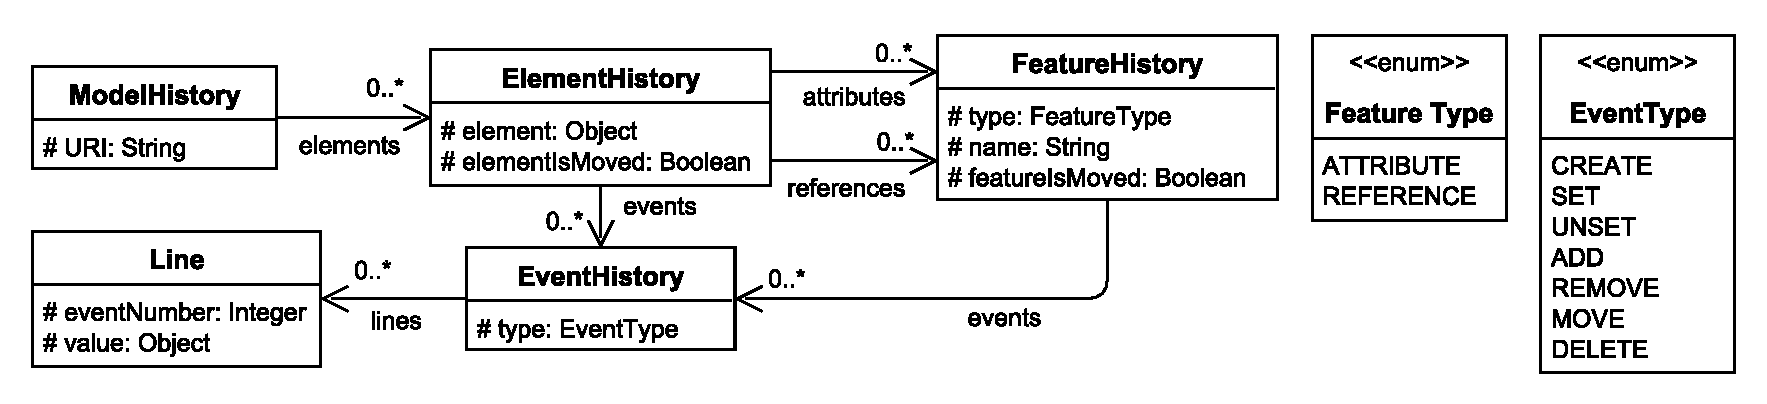
\includegraphics[width=\linewidth]{object_history}
\caption{A class diagram of recording object history.}
\label{fig:object_history}
\end{figure}

To save events captured in Alg. \ref{alg:capture_events}, we follow steps in Alg. \ref{alg:fill_history}. The algorithm requires three input: \emph{modelHistory}, \emph{event}, \emph{lineNumber}.  Inside the procedure \emph{addEventToHistory}, the algorithm starts by retrieving the \emph{object} affected by the occurring event from the \emph{event} using the get \emph{objectFunction} (line 3). The procedure then checks if the \emph{object}'s\emph{objectHistory} does not exists yet in the \emph{modelHistory} (line 4). If it is true then it creates a new one (line 5). If it is false then it retrieves the \emph{objectHistory} from the \emph{modelHistory} (line 7). 

\begin{algorithm}
\begin{small}
\SetKwInOut{Input}{input}
\Input{an object of ModelHistory $modelHistory$, an object of Event $event$, a value of Integer $lineNumber$}
\SetKwProg{Procedure}{procedure}{\\begin}{end}
\Procedure{addEventToHistory($modelHistory$, $event$, $lineNumber$)}{
    $object$ $\leftarrow$ getObject($event$)\;
    \uIf{$object$ does not have $objectHistory$ in $modelHistory$}{
        $objectHistory$ $\leftarrow$ createObjectHistory($object$, $modelHistory$)\;
    }\Else{
        $objectHistory$ $\leftarrow$ getObjectHistory($object$, $modelHistory$)\;
    }
    
    $affectedFeature$ $\leftarrow$ getAffectedFeature($event$)\;  
        \uIf{$affectedFeature$ is Attribute}{
            addEventToAttributeHistory($objectHistory$, $event$, $affectedFeature$, $lineNumber$)\;  
        }\ElseIf{$featureObject$ is Reference}{
            addEventToReferenceHistory($objectHistory$, $event$, $affectedFeature$, $lineNumber$)\;  
    }    
    
    $eventType$ $\leftarrow$ getEventType($event$)\;  
    \uIf{$eventType$ does not have $eventHistory$ in $objectHistory$}{
        $eventHistory$ $\leftarrow$  createEventHistory($eventType$, $objectHistory$)\;
    }\Else{
        $eventHistory$ $\leftarrow$ getEventHistory($eventType$, $objectHistory$)\;
    }
    $value$ $\leftarrow$ getValue($event$)\;
    $line$ $\leftarrow$ createLine($lineNumber$, $value$)\;
    add $line$ to $eventHistory$\;
}
\end{small}
\caption{An algorithm to save events captured in Alg. \ref{alg:capture_events} into a model history.}
\label{alg:fill_history}
\end{algorithm}

Lines 9 to 14 are specified to handle events that modify any feature -- an attribute or a containment reference -- of the object (for example, set a value to an attribute, add an object to a containment reference). From the \emph{event}, we can get the \emph{affectedFeature} using \emph{getAffectedFeature} function. If the \emph{affectedFeature} is attribute then the algorithm executes procedure \emph{addEventToAttributeHistory} (lines 10 and 11). If the \emph{affectedFeature} is reference then the algorithm executes procedure \emph{AddEventToReferenceHistory} (lines 12 and 13). Both \emph{addEventToAttributeHistory} and \emph{AddEventToReferenceHistory} are procedures that works similarly to procedure \emph{addEventToHistory} except that they create and add object history instances, as well as their event histories and lines, for the attribute and reference relationships in Fig. \ref{fig:object_history}. The object history instances represents the history of attributes and references that belongs to an object.

\begin{figure}[ht]
\centering
\includegraphics[width=\textwidth,height=\textheight,keepaspectratio]
%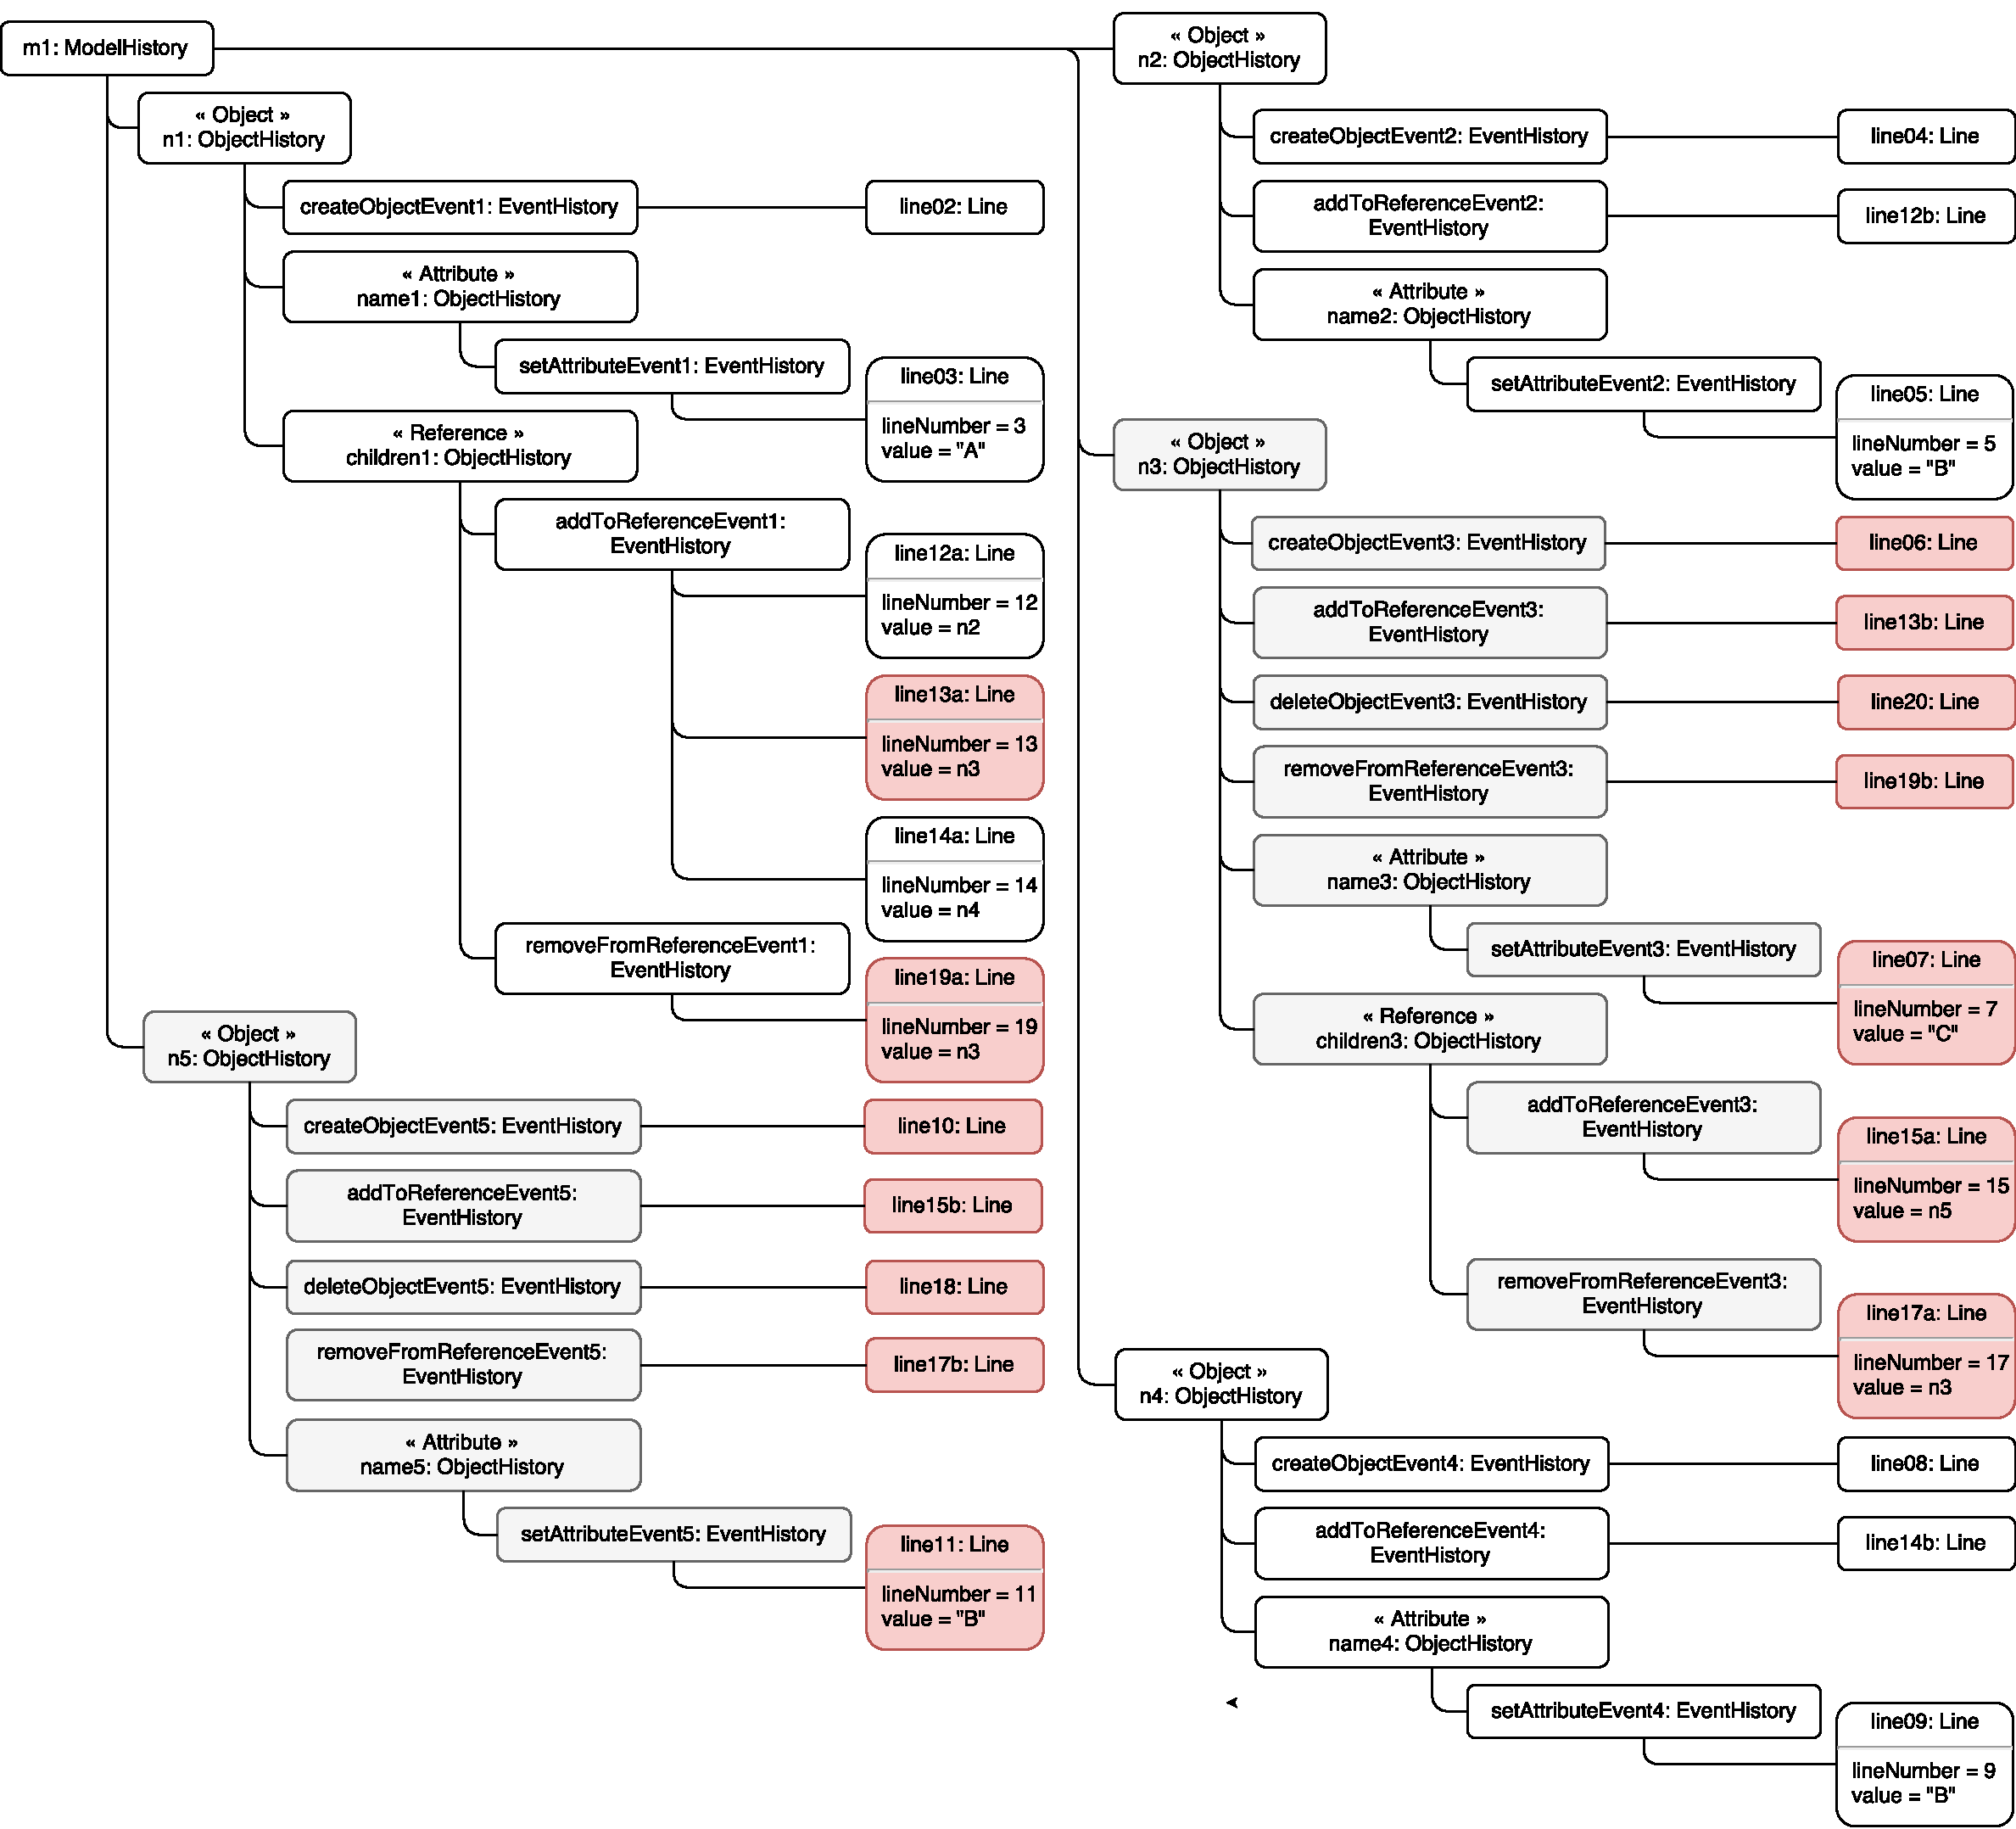
\includegraphics[width=\linewidth]
{history_structure}
\caption{An object diagram showing the structure of object history of the model in Fig. \ref{fig:initial_model}. The red rectangles contain line numbers that are going to ignored when loading CBP.}
\label{fig:history_structure}
\end{figure}

After handling affected features, the algorithm retrieves\emph{eventType} that is held by the \emph{event} using \emph{getEventType} function (line 15). If the \emph{eventType}'s \emph{eventHistory} does not exists in the \emph{objectHistory} then the algorithm creates a new \emph{eventHistory} of the \emph{eventType} in the \emph{objectEvent}  using \emph{createEventHistory} function (lines 16 and 17). Otherwise, it retrieves the \emph{eventHistory} from the \emph{objectHistory} (lines 18 and 19). Using \emph{getValue} function, the algorithm gets any operand's \emph{value} used in the event (the \emph{value} can be null if the event does not use any value) (line 21). The algorithm then uses the \emph{lineNumber}, the \emph{value}, and \emph{createLine} function, to create an instance \emph{line} of class Line and adds it into \emph{eventHistory} (lines 22 and 23).   

The operations that produce Lst. \ref{lst:cbpmodel}, if they are recorded into ModelHistory, yields structure depicted by the object diagram in Fig. \ref{fig:history_structure}. The red rectangles are the Line objects that contain information of line numbers that are going to be ignored when the CBP in Lst. \ref{lst:cbpmodel} is loaded. Some of the objects are collapsed, not displaying the lineNumber field, to save space. Their line numbers are reflected on their object names.  

\section{Loading Time Optimisation}
\label{sec:loading_time_optimisation}
Loading all events to generate the end model of a CBP representation is not efficient, since we can have multiple operations that are cancelled by other operations -- they do not affect the state of the end model. One way to optimise it is by ignoring those operations. Every time an event occurs, we execute algorithms to identify previous events that are cancelled by an event and add them to an ignore list (Alg. \ref{alg:capture_events}, line 6). From the \emph{event} object in Alg. \ref{alg:capture_events}, we can identify what kind of  operations (e.g. create, add, delete) that they represent. With that information, we can perform certain algorithms, utilising the model history in section \ref{sec:model_history}, to identify ignorable lines and put them into the ignore list. We discuss the optimisation of \emph{set} and \emph{unset} operation in subsection \ref{subsec:set_and_unset_operations}, \emph{add}, \emph{remove}, and \emph{move} operations in subsection \ref{subsec:add_remove_and_move_operations}, and \emph{create} and \emph{delete} operations in subsection \ref{subsec:create_and_delete_operations}.

\begin{algorithm}
\begin{small}
\SetKwInOut{Input}{input}
\SetKwInOut{Output}{output}
\Input{a list of Event $eventList$, a list of integer $ignoreList$}
\Begin{
    \ForEach{$event$ in $eventList$}{
        $lineNumber$ $\leftarrow$ getLineNumber($event$)\;
        \If{$lineNumber$ is not in $ignoreList$}{
            replay($event$)\;
        }
    }
}
\end{small}
\caption{CBP loading optimisation algorithm.}
\label{alg:optimised_load}
\end{algorithm}

When a CBP representation is loaded, only events that are not contained in the ignore list that are replayed. In Alg. \ref{alg:optimised_load}, events that are in the \emph{eventList} are iterated one by one (line 2). The \emph{eventList} is loaded from a CBP representation. The algorithm then uses the \emph{getLineNumber} function to get the \emph{lineNumber} of each \emph{event} (line 3). The \emph{lineNumber} then is checked if it does not exist in the \emph{ignoreList} (line 4). If it is true then the \emph{event} is replayed (line 5), otherwise the \emph{event} is ignored.   

\subsection{Set and Unset Operations}
\label{subsec:set_and_unset_operations}
During a model development, an attribute of an object can be assigned many times. We identify that the last value that is assigned to the attribute is all that matters -- the last assigned value is the value that is hold by the attribute in the end model. Previous assignments can be ignored since they do not affect the end version of a model. For example in List. \ref{lst:set_unset_example}, the attribute \emph{name} is assigned \emph{"A"}, and then \emph{"B"}, and then nullified (unset), and finally \emph{"C"}. We can execute only the last assignment (line 5) to optimise the execution, ignoring the previous operations, to produce the same end model as if we executes all the operations. 

\begin{lstlisting}[style=eol,caption={Example of CBP representation of \emph{name} attribute assignments.},label=lst:set_unset_example]
create node of Node
set node.name to "A"    //node.name="A"    
set node.name to "B"    //node.name="B"
unset node.name         //node.name=null
set node.name to "C"    //node.name="C"
\end{lstlisting}

To make the optimisastion possible, the line numbers where the attribute \emph{name} affected in Lst. \ref{lst:set_unset_example} are stored into its respective object history.  For example, lines for \emph{set} and \emph{unset} events in their event histories are \emph{setEventHistory.lines = setEventLines = [[2, "A"], [3, "B"], [5, "C"]]} and \emph{unsetEventHistory.lines = unsetEventLines = [[4, null]]} respectively. Since only the last value of set or unset operations that is significant, using the two lists, we can identify that line 5 is the last line of set and unset operations that is significant for the attribute \emph{name}. Therefore, lines 2 to 4 can be put into the ignore list.  

\begin{algorithm}
\begin{small}
\SetKwInOut{Input}{input}
\SetKwInOut{Output}{output}
\SetKwProg{Struct}{struct}{}{end}
\Struct{Line}{
    Integer $lineNumber$;
    Var $value$;
}
\Input{two lists of Line $setEventLines$ and $unsetEventLines$, a list of Integer $ignoreList$}
\Output{a list of Integer $ignoreList$}
\SetKwBlock{Beginn}{beginn}{ende}
\Begin{
$setLastLine$ $\leftarrow$ getLastLine($setEventLines$)\;
$unsetLastLine$ $\leftarrow$ getLastLine($unsetEventLines$)\;
\uIf{$setLastLine > unsetLastLine$}{
    Add every line number in $setEventLines$ into $ignoreList$ except the last line\;
    Add all line numbers in $unsetEventLines$ into $ignoreList$\; 
}

\ElseIf{$setLastLine < unsetLastLine$}{
    Add all line numbers in $setEventLines$ into $ignoreList$\;
    Add all line numbers in in $unsetEventLines$ into $ignoreList$\; 
}
\Return{$ignoreList$}\;
}
\end{small}
\caption{Algorithm to identify lines that can be ignored for attribute's \emph{set} and \emph{unset} operations}
\label{alg:set_unset_optimisation}
\end{algorithm}

The algorithm to execute this argument is shown in Alg. \ref{alg:set_unset_optimisation}. It takes three inputs: two list of \emph{Line}, \emph{setEventLines} and \emph{unsetEventLines}, and a list of Integer, \emph{ignoreList}. The \emph{Line} is a structure that represents an event. It carries the \emph{lineNumber} of the event in its CBP representation as well as the \emph{value} involved. The \emph{setEventLines} and \emph{unsetEventLines} are lists that contains the \emph{Line}s where the event \emph{setAttributeEvent} and \emph{unsetAttributeEvent} appear in a CBP representation and the operand's value included in the event. The algorithm starts by retrieving the last lines of \emph{setEventLines} and \emph{unsetEventLines} using the \emph{getLastLine} function and assigning them to variables \emph{setLastLine} and \emph{unsetLastLine} (lines 5 and 6). If \emph{setLastLine} is larger than \emph{unsetLastLine} then every line number that is in the \emph{setEventLines} are put into the \emph{ignoreList} excluding the last value since the last line still has to be executed to produce the same end model (lines 7-9). If \emph{unsetLastLine} is larger than \emph{setLastLine} then \emph{unset} operation is the last operation that is executed (line 10). Therefore, there is no need to executes all \emph{set} and \emph{unset} operations -- all lines can be ignored. Every line numbers in \emph{setEventLines} and \emph{unsetEventLines} are put into the \emph{ignoreList}. The \emph{ignoredList} is then returned for further processes.

The algorithm (Alg. \ref{alg:set_unset_optimisation}) can also be applied to set and unset operations of a containment reference for CBP described in Lst. \ref{lst:set_unset_reference}. For nodes \emph{n1}, \emph{n2}, \emph{n3}, and \emph{n4} are created at the beginning of the creation of its model (line 1-4). The \emph{n1}'s single containment reference, \emph{associate}, is then assigned \emph{n2} and \emph{n3} accordingly (lines 5-6), before nullified or unset (line 7). Finally, the \emph{n1.associate} is set to \emph{n4}. 

\begin{lstlisting}[style=eol,caption={Example of CBP representation of \emph{name} reference assignments.},label=lst:set_unset_reference]
create n1 of Node
create n2 of Node
create n3 of Node
create n4 of Node
set n1.associate to n2    //node.associate=n2
set n1.associate to n3    //node.associate=n3
unset n1.associate        //node.associate=null
set n1.associate to n4    //node.associate=n4
\end{lstlisting}

Using the same optimisation to set and unset operations of containment reference \emph{associate}, we can omit lines 5 to 7 to produce the same end model. In in their event histories, the lines for set and unset operations are \emph{setEventLines = [[5, n2], [6, n3], [8, n4]]} and \emph{unsetEventLines = [[7, null]]} respectively. Since only the last value of set or unset operations that is significant, using the two lists, we can identify that line 8 is the last line of set and unset operations that is significant for the containment reference \emph{associate}. Therefore, lines 5 to 7 can be put into the ignore list.

\subsection{Add, Remove, and Move Operations}
\label{subsec:add_remove_and_move_operations}
An attribute can also contains many values; we can add remove values from it. For example (List. \ref{lst:add_remove_attribute_literal_example}), \emph{node} object has \emph{values} attribute that can contains many integer values. We add values 11, 12, and 13 subsequently (line 2-4) to the attribute and remove the value 12 at line 5. We show in the commented parts the states of \emph{node.values}.  

\begin{lstlisting}[style=eol,caption={Example of CBP representation of attribute \emph{values}'s add and remove operations.},label=lst:add_remove_move_attribute]
create node of Node
add 11 to node.values      //node.values=[11] 
add 12 to node.values      //node.values=[11,12] 
add 13 to node.values      //node.values=[11,12,13] 
remove 12 from node.values //node.values=[11,13] 
\end{lstlisting}

The execution of these operations can be optimised by ignoring the add and remove operations of the value 12 (lines 3 and 5) since we can produce the same end model only by adding 11 and 13 (line 2, 4). When events in List. \ref{lst:add_remove_move_attribute} are executed, they populate line lists for add and remove event histories of attribute \emph{values}, \emph{addEventLines = [[2,11], [3,12], [4,13]]} and \emph{removeEventLines = [[5,12]]}. Using the two lists, we can identify the line number of lines that can be put into the ignore list, producing \emph{ignoreList = [3, 5]}. The algorithm to execute this argument is shown in Alg. \ref{alg:add_remove_move_optimisation}.

\begin{algorithm}
\begin{small}
\SetKwInOut{Input}{input}
\SetKwInOut{Output}{output}
\SetKwProg{Struct}{struct}{}{end}
\Struct{Line}{
    Integer $lineNumber$;
    Anytype $value$;
}
\Input{two lists of Line $addEventLines$, $removeEventLines$, and $moveEventLines$, a list of Integer $ignoreList$, a variable of Anytype $operandValue$, a variable of Boolean $attributeIsMoved$, an object of Feature $feature$}
\Output{a list of Integer $ignoreList$}
\SetKwBlock{Beginn}{beginn}{ende}
\Begin{
\If{$attributeIsMoved$ = false}{
    $filteredAddLines$ $\leftarrow$ filterLinesByValue($addEventLines$, $operandValue$)\;
$filteredRemoveLines$ $\leftarrow$ filterLinesByValue($removeEventLines$, $operandValue$)\;
$addLastLine$ $\leftarrow$ getLastLine($filteredAddLines$)\;
$removeLastLine$ $\leftarrow$ getLastLine($filteredRemoveLines$)\;
\uIf{$addLastLine > removeLastLine$}{
    Add every line number in $filteredAddLines$ into $ignoreList$ except the last value\;
    Add all line numbers in $filteredRemoveLines$ into $ignoreList$\; 
}
\ElseIf{$addLastLine < removeLastLine$}{
    Add all line numbers in $filteredAddLines$ into $ignoreList$\;
    Add all line numbers in $filteredRemoveLines$ into $ignoreList$\; 
}
}
\If{feature is empty or feature only has a value}{
    \uIf{feature is empty}{
        Add all line numbers in $addEventLines$ into $ignoreList$\;
    }\ElseIf{feature only has a value}{
        Add every line number in $addEventLines$ into $ignoreList$ except the last value\;
    }
        Add all line numbers in $removeEventLines$ into $ignoreList$\; 
        Add all line numbers in $moveEventLines$ into $ignoreList$\; 
        $attributeIsMoved$ $\leftarrow$ false\;
}
\Return{$ignoreList$}\;
}
\end{small}
\caption{Algorithm to identify lines that can be ignored for \emph{add}, \emph{remove}, and \emph{move} operations.}
\label{alg:add_remove_move_optimisation}
\end{algorithm}

The algorithms takes seven inputs: three line lists -- addEventLines, removeEventLines, and moveEventLines -- that contain the lines of add, remove, and move events, an ignore list \emph{ignoreList}, the variable \emph{operandValue} to hold the value used in an event, a flag variable \emph{attributeIsMoved}, and an object of Feature \emph{feature} which can be an attribute or containment reference. The algorithm starts by checking the value of \emph{attributeIsMoved} to the member of the attribute's values if they are already moved or not (line ). We explain more the use of \emph{attributeIsMoved} later in this section. If the values are not moved yet, the algorithm continues with filtering all the line lists by the operandValue and stored them into filtered line lists: \emph{filteredAddLines} and \emph{filteredRemoveLines}. The algorithm the retrieves the last lines of the filtered line lists using the \emph{getLastLine} function and assigns them to \emph{addLastLine} and \emph{removeLastLine}. If the \emph{addLastLine} is larger than {removeLastLine} then all line numbers of {\emph{filteredAddLines} and \emph{filteredRemoveLines}, except for the last line of \emph{filteredAddLines}, are added into the \emph{ignoreList}. Otherwise, all line numbers in both filtered line lists are added into the\emph{ignoreList}.

The algorithm then proceeds by checking the feature. If the feature is empty then all line numbers in the \emph{addEventLines} are added into the \emph{ignoreList}. If the feature only has one value, all the line numbers also added into the \emph{ignoreList} except the last line. The algorithm then proceeds by adding all line numbers in \emph{removeEventLines} and \emph{moveEventLines} into the \emph{ignoreList}. After that, \emph{attributeIsMoved} is set to false. Finally, the \emph{ignoreList} is returned for further operations.    

\begin{lstlisting}[style=eol,caption={Example of CBP representation of attribute \emph{values}'s add and remove operations.},label=lst:add_remove_move_reference]
create n1 of Node
create n2 of Node
create n3 of Node
create n4 of Node
add n2 to node.children      //n1.children=[n2] 
add n3 to node.children      //n1.children=[n2,n3] 
add n4 to node.children      //n1.children=[n2,n3,n4] 
remove n3 from node.children //n1.children=[n1,n4] 
\end{lstlisting}

The algorithm (Alg. \ref{alg:add_remove_move_optimisation}) can also be applied to add, remove, and move operations of a containment reference for CBP described in Lst. \ref{lst:add_remove_move_reference}. For nodes \emph{n1}, \emph{n2}, \emph{n3}, and \emph{n4} are created at the beginning of the creation of its model (line 1-4). The \emph{n1}'s multivalue containment reference, \emph{children}, is then added \emph{n2},\emph{n3}, and \emph{n4} accordingly (lines 5-7), before the removal of node \emph{n3} (line 8). 

Using the same optimisation to \emph{add}, \emph{remove}, and \emph{move} operations of containment reference \emph{children}, we can omit lines 6 to 8 to produce the same end model. In in their event histories, the lines for set and unset operations are \emph{addEventLines = [[5, n2], [6, n3], [7, n4]]} and \emph{removeEventLines = [[8, n3]]} respectively. Since the \emph{remove} operation at line 8 makes itself and the \emph{add} operation at line 6 insignificant, lines 6 and 8 can be put into the ignore list.

\begin{lstlisting}[style=eol,caption={Example of CBP representation of attribute \emph{values}'s move operations.},label=lst:move_attribute_example]
create node of Node
add 11 to node.values            //node.values=[11] 
add 12 to node.values            //node.values=[11,12] 
add 13 to node.values            //node.values=[11,12,13] 
move from 0 to 1 in node.values  //node.values=[12,11,13]  
remove 12 from node.values       //node.values=[11,13] 
\end{lstlisting}

\begin{lstlisting}[style=eol,caption={Example of optimised CBP representation of attribute \emph{values}'s move operations.},label=lst:move_attribute_example_error]
create node of Node              //(1)  
add 11 to node.values            //(2) node.values=[11] 
add 13 to node.values            //(4) node.values=[11,13] 
move from 0 to 1 in node.values  //(5) node.values=[13,11]   
\end{lstlisting}

The `\emph{if attributeIsMoved = false}' condition at line 5 in Alg. \ref{alg:add_remove_move_optimisation} indicates that removing previous add and remove events can only be applied if no move operation has been executed previously to the attribute. This condition is required, since after optimisation, some operations are already removed and therefore makes some values may not exist, which changing the indexes of other values. Consequently, replaying all the events may not produce the same end model with the non-optimised CBP representation. 

To illustrate this case, we compare the end model loaded from a CBP representation (List. \ref{lst:move_attribute_example}) to another model loaded from and optimised CBP representation (List. \ref{lst:move_attribute_example_error}) -- the same representation but has been optimised. The optimisation removes line 3 and 6 in List. List. \ref{lst:move_attribute_example} and when loaded back again the end models are not same. The non-optimised CBP representation produces \emph{node.values=[11,13]} while the optimised one produces \emph{node.values=[13,11]}. When \emph{remove 12} is executed (List. \ref{lst:move_attribute_example} line 6), the optimisation ignores the \emph{add 12} operation (List. \ref{lst:move_attribute_example} line 3) and thus makes the index of 13 is 1 in the optimised CBP, while the index of 13 is 2 in the non-optimised CBP, and produces different end model when \emph{move from 0 to 1} (List. \ref{lst:move_attribute_example_error} line 4) is executed. 

The \emph{attributeIsMoved}'s state is set to true when a move operation is applied within it's attribute and the number of of it's attributes' values is more than 1. The \emph{attributeIsMoved}'s state is set to false again when the attribute is empty or only has a value (\ref{alg:add_remove_move_optimisation}, line 18-26) since any move operation does not affect the indexes of the attributes' values.



%\begin{lstlisting}[style=eol,caption={Example of CBP representation of attribute \emph{values}'s move operations.},label=lst:move_attribute_object_example]
%create node of Node
%create n1 of Node
%create n2 of Node
%create n3 of Node
%add n1 to node.children            //node.children=[n1] 
%add n2 to node.children            //node.children=[n1,n2] 
%add n3 to node.children            //node.children=[n1,n2,n3] 
%move from 0 to 1 in node.children  //node.children=[n2,n1,n3]  
%remove n2 from node.children       //node.children=[n1,n3] 
%\end{lstlisting}
%
%\begin{lstlisting}[style=eol,caption={Example of optimised CBP representation of attribute \emph{values}'s move operations.},label=lst:move_attribute_example_object_error]
%create node of Node                //(1)  
%create n1 of Node                  //(2)  
%create n3 of Node                  //(4)  
%add n1 to node.children            //(5) node.children=[n1] 
%add n3 to node.children            //(7) node.children=[n1,n3] 
%move from 0 to 1 in node.children  //(8) node.children=[n3,n1]   
%\end{lstlisting}

\subsection{Create and Delete Operations}
\label{subsec:create_and_delete_operations}
The examples of object's create event has been demonstrated in several Listings in this paper where \emph{create} is the keyword that denotes the event in a CBP representation. The create operation is only executed  once per object. It cannot be created more than once. Meanwhile, the example of object's delete event is exhibited in Lst. \ref{lst:cbpmodel}. When an object is deleted, it means that the object is completely removed from the model -- no longer exists. Therefore, all events (create, delete, set, unset, add) related to the object can be ignored -- there is no need to create the object and all its attributes' events can be ignored as well. 

If  Lst. \ref{lst:cbpmodel} is optimised by removing node n3 (n5 is removed first since n5 is contained in n3), then the otimisation produces the CBP representation as in Lst. \ref{lst:cbpmodel_optimised}. The optimisation ignores 10 lines (lines 6, 7, 10, 11, 13, 15, 17, 18, 19, and 20) since those lines are related to nodes \emph{n3} and \emph{n5} and ignoring the lines still produces the same end model to the one produced by the non-optimised CBP representation (Lst. \ref{lst:cbpmodel}). 

\begin{lstlisting}[style=eol,caption={Change-based representation of the model of Figure \ref{fig:initial_model} after removal of node \emph{n5}.},label=lst:cbpmodel_optimised]
session s1                   //(1)
create n1 of Node            //(2)
set name of n1 with "A"      //(3)  n1.name="A"
create n2 of Node            //(4)
set name of n2 with "B"      //(5)  n2.name="B"
create n4 of Node            //(8)
set name of n4 with "D"      //(9)  n4.name="D"
add n2 to n1.children        //(12) n1.children={n2}
add n4 to n1.children        //(14) n1.children={n2,n4}
session s2                   //(16)
\end{lstlisting}

We use Alg. \ref{alg:create_delete} to determine lines that are ignored after a \emph{delete} operation. The algorithm takes two inputs, \emph{deletedObject}, an variable of object that is deleted, and \emph{ignoreList}, a list of Integer that contains ignored line numbers. After some processes, the algorithm will return the \emph{ignoreList} as its output. The algorithm starts by checking whether the \emph{deletedObject} is already moved or not (line 2), if it is not then it is safe to remove all lines that refer to the object (line 3). Otherwise, no action is executed. The algorithm then retrieves all event histories \emph{eventHistoryList} that refer to the object (line 4)and iterates through each event history (line 5-8). For every event history \emph{eventHistory} (line 5), the algorithm retrieves its lines \emph{lineList} (line 6) and put all their line numbers into the \emph{ignoreList} (line 7). After that, the algorithm continues to iterate through all its attributes and put all lines of their events into the \emph{ignoreList} as well (lines 12-15). As a result, the next time the CBP representation (Lst. \ref{lst:cbpmodel}) is loaded, the loading process can refer to the \emph{ignoreList} whether certain lines in the CBP representation are ignored or not.       

\begin{algorithm}
\begin{small}
\SetKwInOut{Input}{input}
\SetKwInOut{Output}{output}
\Input{a variable ofObject $deletedObject$, a list of Integer $ignoreList$}
\Output{a list of Integer $ignoreList$}
\Begin{
$objectIsMoved$ $\leftarrow$ isObjectMoved($deletedObject$)\;
\If{$objectIsMoved$ = false}{
    $eventHistoryList$ $\leftarrow$ getAllEventHistories($deletedObject$)\; 
    \ForEach{$eventHistory$ in $EventHistoryList$}{
        $lineList$ $\leftarrow$ getLines($eventHistory$)\;
        Add all line numbers in $lineList$ into $ignoreList$\; 
    }
    $attributeList$ $\leftarrow$ getAllAttributes($deletedObject$)\;
    \ForEach{$attribute$ in $attributeList$}{
        $eventHistoryList$ $\leftarrow$ getAllEventHistories($attribute$)\;
        \ForEach{$eventHistory$ in $EventHistoryList$}{
            $lineList$ $\leftarrow$ getLines($eventHistory$)\;
            Add all line numbers in $lineList$ into $ignoreList$\; 
        }       
    }   
}
\Return{$ignoreList$}\;
}
\end{small}
\caption{Algorithm to identify lines that are ignored after \emph{delete} operations}
\label{alg:create_delete}
\end{algorithm}

For example, based on Lst. \ref{lst:cbpmodel} and Fig. \ref{fig:history_structure}, at the moment when node \emph{n5} is deleted, it already had 5 instances of \emph{eventHistory}: 4 instances (\emph{createObjectEvent5}, \emph{addToReferenceEvent5}, \emph{deleteObjectEvent5}, and \emph{removeFromReferenceEvent5}) that are contained directly in its object history and 1 instance (\emph{setAttributeEvent5}) is contained in its attribute \emph{name} object history. Those instances has line lists that contain line numbers as follows: \emph{createObjectEvent5.lines = [[10]]}, \emph{addToReferenceEvent5.lines = [[15]]}, \emph{deleteObjectEvent5.lines = [[18]]}, and \emph{removeFromReferenceEvent5.lines = [[17]]}, \emph{setAttributeEvent5.lines = [[11, "B"]]}. Using Alg. \ref{alg:create_delete}, deleting node \emph{n5} means filling the \emph{ignoreList} with all the line numbers contained by its event histories. Thus, the deletion produces \emph{ignoreList = [10, 11, 15, 17, 18]}. Using the same approach, the deletion of node n3 adds more line numbers and produces \emph{ignoreList = [6, 7, 10, 11, 13, 15, 17, 18, 19, 20]}.

\section{Performance Evaluation}
\label{sec:performance_evaluation}
We have implemented a prototype\footnote{The prototype is available under \url{https://github.com/epsilonlabs/emf-cbp}} of the change-based model persistence using the Eclipse Modelling Framework. We evaluate the prototype's performance on saving and loading time. For the saving time, we contrast the saving time between appending in CBP and saving in XMI. For the loading time, we perform comparison on loading time between optimised CBP, non-optimised CBP, and XMI.

\subsection{Saving Time Test}
\label{subsec:saving_time_test}
We test the performance of our prototype on saving time to gain insight on the efficiency that can be gained from the CBP representation against XMI, a common standard for model serialisation, as the comparison baseline. The  comparison is depicted in Fig. \ref{fig:append_speed}.

\begin{figure}[ht]
\centering
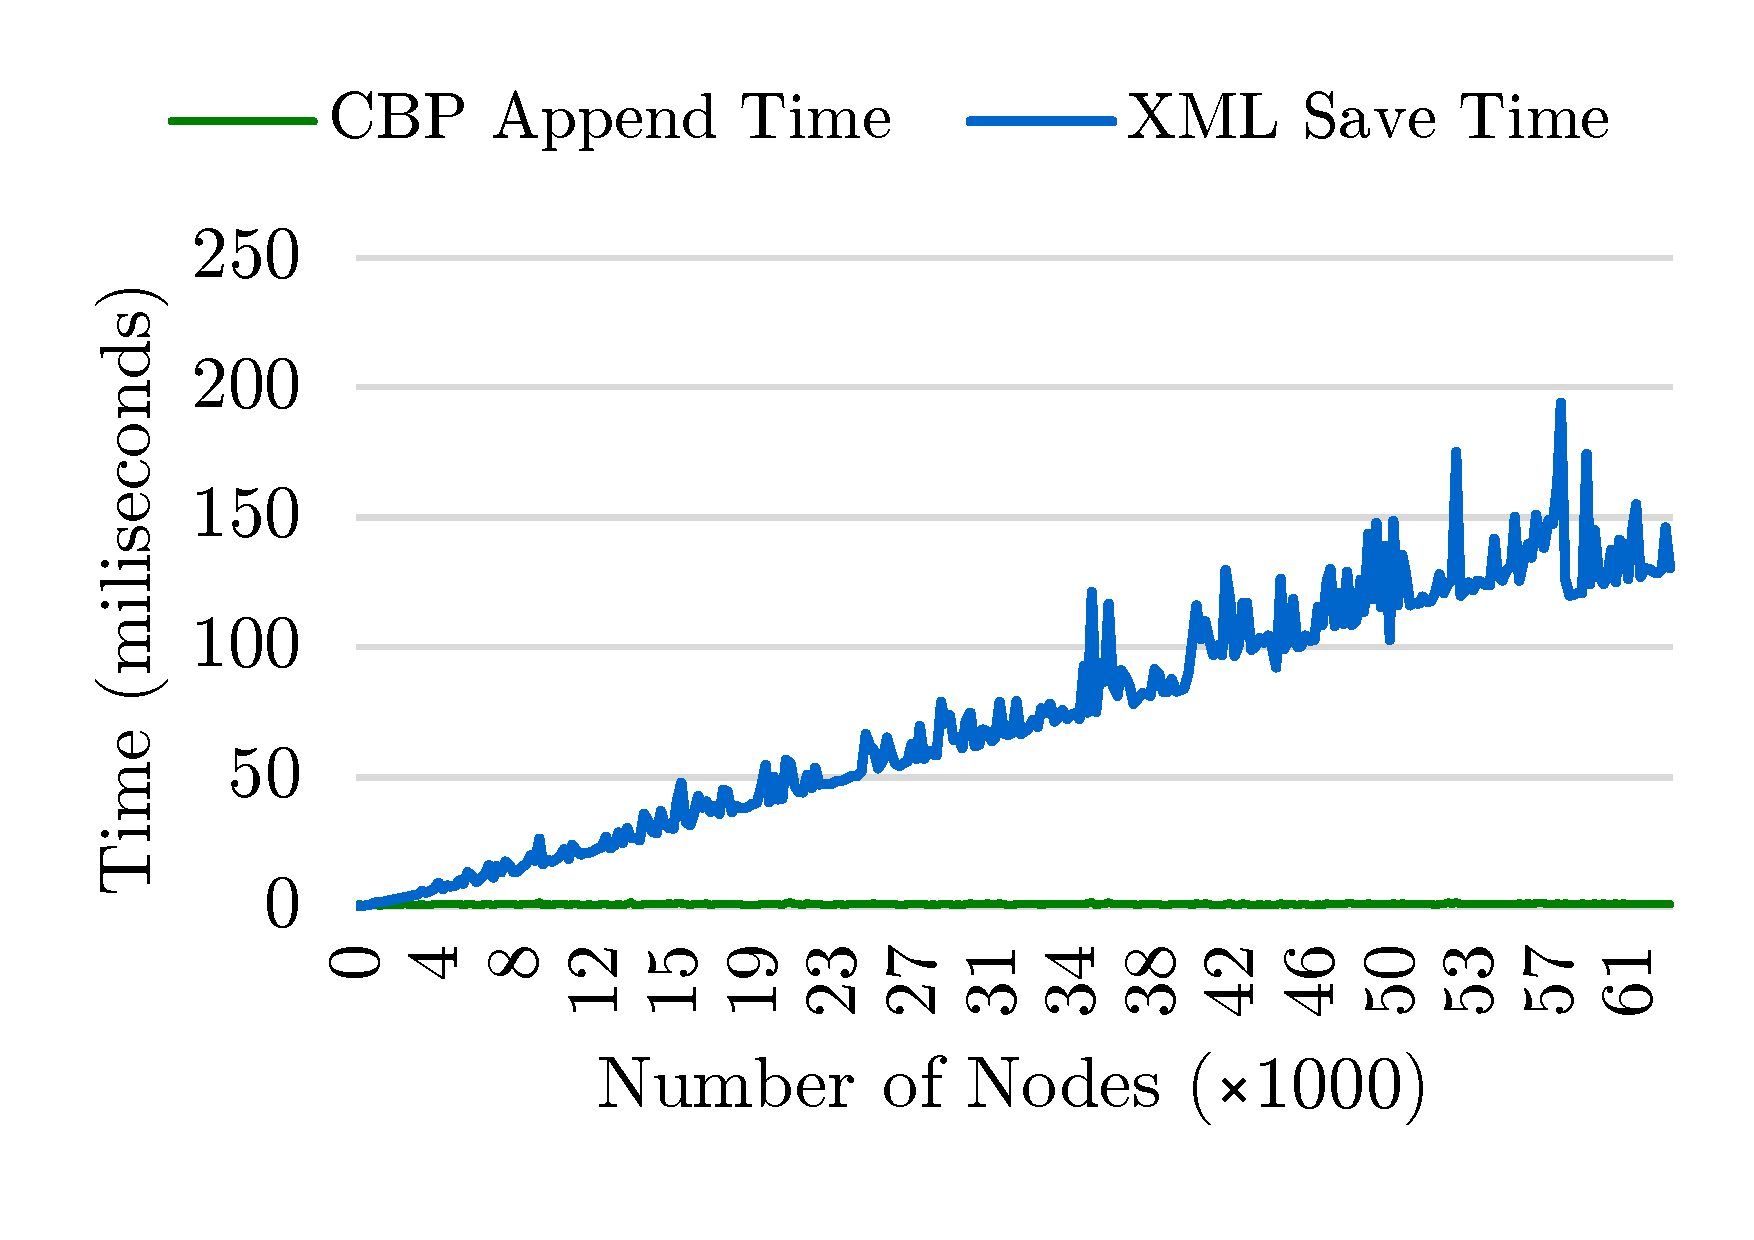
\includegraphics[width=\linewidth]{append_speed}
\caption{A comparison on time used to persist models between CBP (CBPAppend) and XMI (XMISave).}
\label{fig:append_speed}
\end{figure}

In performing our comparison, we seek the relationship between number of nodes and time required to all the nodes. We create a course of random operations in building a model. 
Firstly, we create 10 nodes as the initialisation of the model and to facilitate other types operations, other than \emph{create} operation, to be executed (if there is no node, other types operations cannot be executed). The succeeding operations are randomly selected from a set of possible operation types, which are \emph{set attribute}, \emph{unset attribute}, \emph{add attribute value}, \emph{move attribute value}, \emph{remove attribute value}, \emph{add object value}, \emph{move object value}, \emph{create object}, and \emph{delete object}. The probability of occurrence of the types are set to ratio 1:1:3:2:1:3:2:2:1 respectively. As an example, based on the ratio, the probability for \emph{delete object} operation to occur is 1/16 for each iteration. The ratio of  \emph{create} operation has to be set larger than \emph{delete} operation to ensure the model grows -- to have more nodes.  

Every time each operation is executed, we append the event of the operation into the CBP representation as well as save the state of the model at that time into an XMI. We measure the time consumed for each of the append and save operations. Every time the number of the nodes reach the fold of 200 (200, 400, 600, and so on), we record the the time required and plot them into a linechart as depicted in Fig. \ref{fig:append_speed}.

In the Fig. \ref{fig:append_speed}, we can notice that persisting the model by appending changes into the CBP representation works in a constant time along the growth of the model. The average time required to append an event of an operation is \emph{AVG} = 0.99 ms with standard deviation \emph{SD} = 0.16 ms. In contrast, persisting the end state of the whole model consumes more time every time the model grows. When the model reach 47,800 nodes, the time consumed to save the model as an XMI is 107.59 ms, which is around 108.68 times slower than CBP at that number of nodes. 

\subsection{Loading Time Test}
\label{subsec:loading_time_test}
We test the performance of our prototype on loading time to gain insight on efficiency that can be gained with the optimisation algorithms. We do comparison on loading speed between optimised CBP and non-optimised CBP, and also with XMI as the baseline. The  comparison is depicted in Fig. \ref{fig:loading_speed}.

\begin{figure}[ht]
\centering
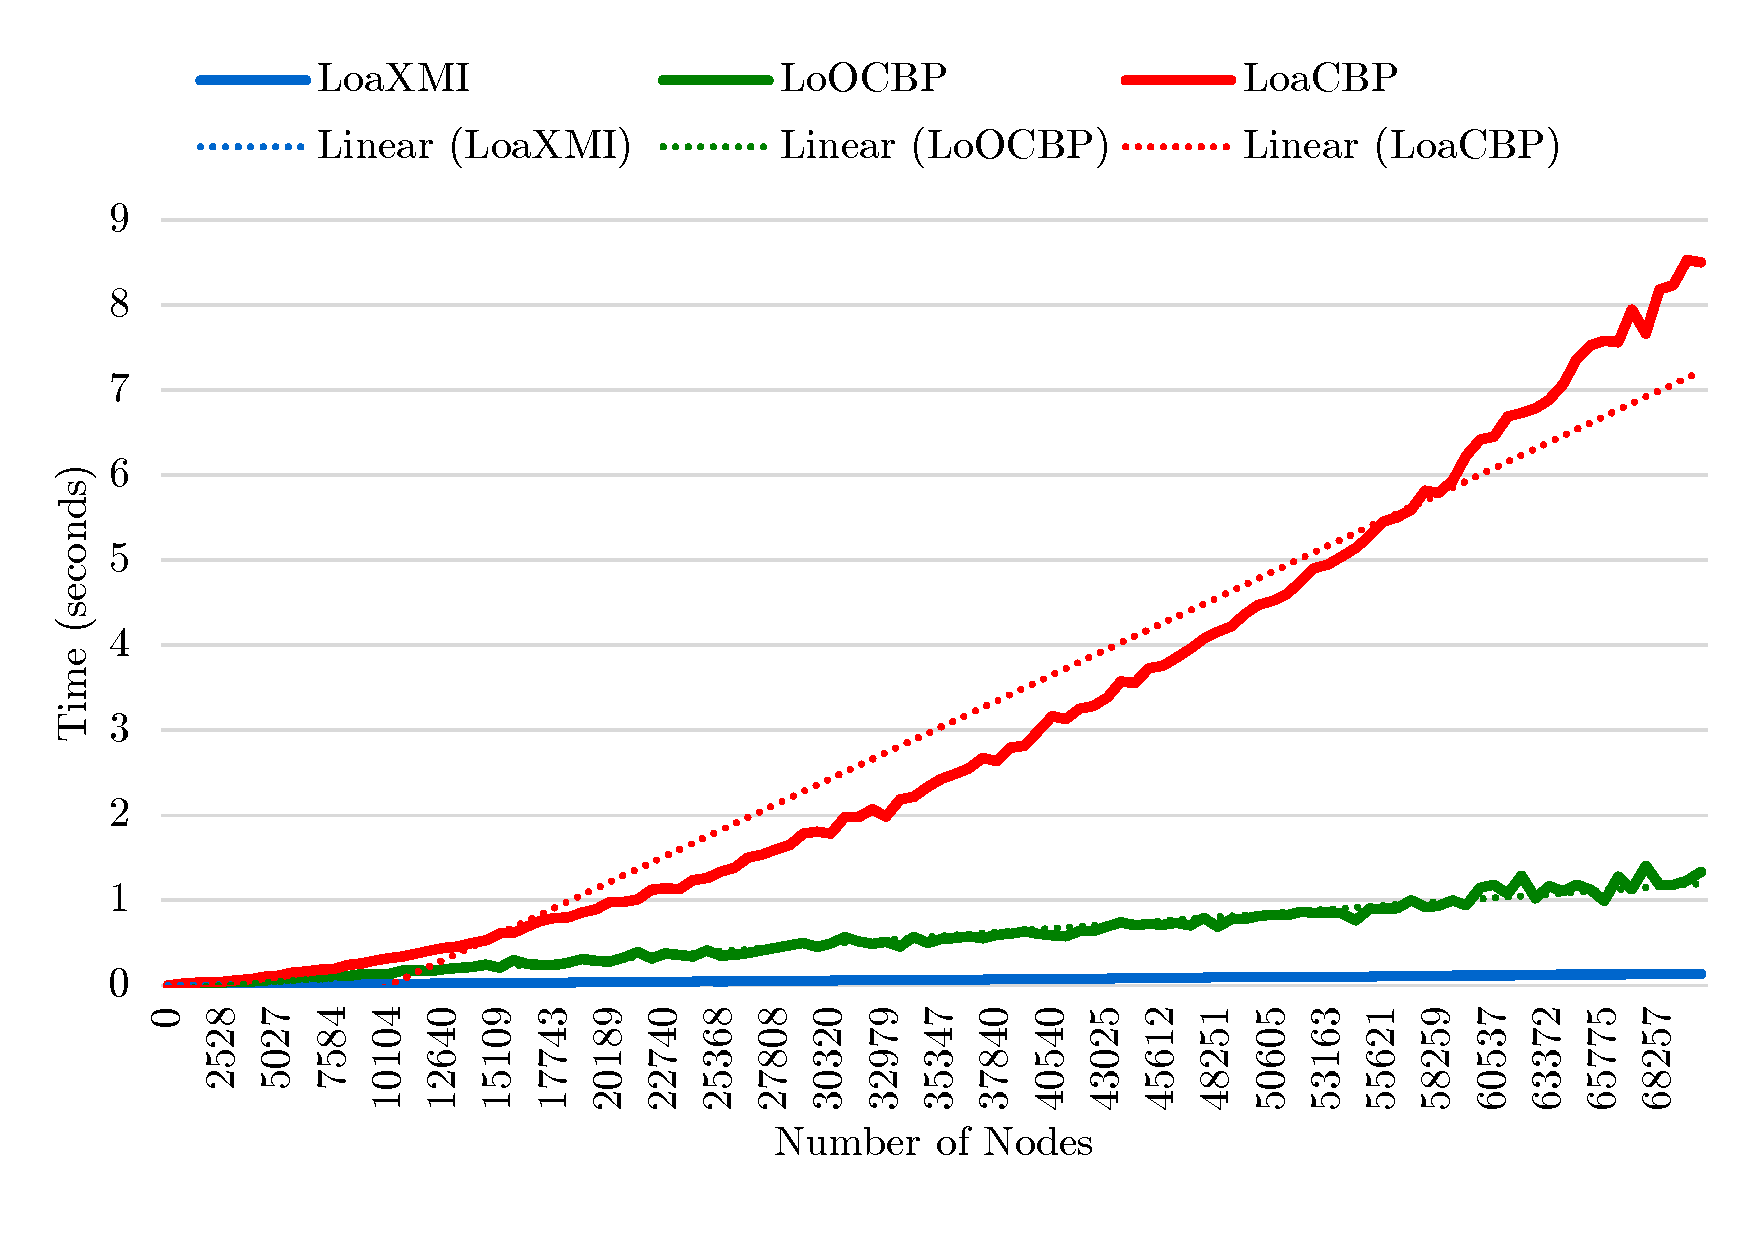
\includegraphics[width=\linewidth]{loading_speed}
\caption{A comparison on loading time between XMI (LoaXMI), optimised CBP (LoOCBP), and non-optimised CBP (LoaCBP).}
\label{fig:loading_speed}
\end{figure}

In performing our comparison, we seek the relationship between number of nodes and time required to all the nodes. The number of nodes increases each time we perform measurement. We perform an iterative measurement that starts with an empty model -- no node exists -- and then increases the number of nodes by 500 for each succeeding iteration until the number reaches 55,500. In each iteration, first, initial nodes are populated as many as the number of nodes for that iteration. 

The model then goes through an alteration process, a process that randomly manipulates the model with a number of different operations. The number of operations is as many as the initial number of nodes. So if the initial number of nodes is 1000 then the number of succeeding operations is 1000. The type of each operation is also randomly selected from a set of possible operation types, which are \emph{set attribute}, \emph{unset attribute}, \emph{add literal value}, \emph{move literal value}, \emph{remove literal value}, \emph{add object value}, \emph{move object value}, \emph{create object}, and demph{delete object}. The probability of occurrence of the types are set to ratio 1:1:3:2:1:3:2:1:1 respectively. 

The population of the initial nodes and the alteration are then serialised as an Epsilon Object Language (EOL) script \cite{kolovos2006epsilon}. This serialisation makes the same produced script to be used across different loading time tests: loading XMI, optimised CBP, and non-optimised CBP. Including create and delete operations in the succeeding operations makes the number of nodes at the end of each alteration possible to be different from the number of the initial nodes. Thus, we can identify in Fig. \ref{fig:loading_speed} that values in x-axis are not exactly the multiple of 500.    

Fig. \ref{fig:loading_speed} shows that the non-optimised CBP consumes more time than XMI and optimised CBP in loading model. It follows an exponential pattern along the increment of nodes. Our optimisation is proven that optimised CBP is becoming more efficient when the number of loaded nodes is increasing. However, still, it cannot outperform the XMI's loading time, since more time is used to de-serialise the CBP format. Optimising the serialised format is possibly will reduce the loading time. From our simulation, with the specification of probability of random operations mentioned previously, the average loading time of optimised CBP is \emph{AVG} = 7.84 (\emph{SD} = 1.47) times slower in than XMI's loading time. Although it is slower, the loading time for 70,271 nodes is only a bit more than one second which is tolerable for a user when loading a model in a modelling application. 

However, models in the real world are most likely different from the random models generated in our loading time testing since real-world models have their own unique characteristics. Thus, the loading time are vary across different models. The optimised CBP may perform better or worse than the one presented in this paper. Moreover, the optimised CBP is not always out perform the non-optimised CBP in every condition. There is condition where optimised CBP is not faster than the non-optimised CBP that is when only \emph{create} operation is performed -- no other types of operations, since there is no event that can be ignored. 

\section{Limitations}
\label{sec:limitations}
So far, we only address feature -- attribute or reference -- that can only contains unique members -- no duplicate values or objects. Duplicate members means that removal of a value /object does not mean the removal of other same values/objects since values/objects with different positions contained in the feature are perceived as different entity. Therefore, positions of values/objects have to be taken into account as well by the optimisation algorithm. We also only address containment reference -- deletion of an object will also delete its contained objects -- which is very different from the non-containment one that the deletion of an object does not delete its contained objects. The deletion has to identify non-containment reference so the creation events objects that are referenced should not be ignored. Furthermore, we also have not address features that has default values. Default value of a feature might not trigger any event. Failure to address this might produce different end models. 

Moreover, the loading test performed might not reflect the CBP of the construction of real-world models. Each model has its own development characteristics and one feasible way to capture them is to ask modellers to create complex models using different modelling languages, persist their histories, and analyse the results to gain insight whether the optimisation really works for real-world models. 

\section{Conclusions}
\label{sec:conclusions}
In this paper, we have proposed a change-based, as an alternative to stated-based, persistence as an approach to persist a model. The persistence enables high-performance processing (e.g. transformation, validation) for incremental model by reducing the change identification cost of evolving models. We have illustrated our approach in implementing the persistence as well as its optimisation algorithms to improve its loading time. Based on our performance test on model loading time, optimised change-based persistence outperforms its unoptimised version. However, even though it still cannot outperform the stated-based persistence's loading time, it operates in the range of time that is still tolerable for users. 

For future work, persisting models in a change-based format means that model files will keep growing in size during their evolution significantly faster than their state-based counterparts. To address this challenge, (1) we will propose sound change-compression operations (e.g. remove older/unused information) that can be used to reduce the size of a model in a controlled way. (2) We will develop a compact textual format that will minimise the amount of space required to record a change (a textual line-separated format is desirable to maintain compatibility with file-based version control systems). (3) We will propose a hybrid model persistence format which will be able to incorporate both change-based and state-based information. 

%For the proposed approach to have a strong practical impact, it needs to be supported by modelling, model processing (e.g. transformation) languages, and model management (e.g. comparison, differencing, merging) tools. To address this challenge, (1) We will extend existing open-source graphical editor frameworks such as Sirius\footnote{\url{http://eclipse.org/sirius/}}, GMF\footnote{\url{http://www.eclipse.org/gmf-tooling/}}, and Papyrus\footnote{\url{http://eclipse.org/papyrus/}} so that they can support the development of editors that persist models in the proposed change-based format. (2) We will extend open-source model processing languages so that they can incrementally process change-based models. We will initially target languages of the well-established Epsilon family, which the PI is leading, but we will explore how other languages that already support incremental execution (e.g. OCL, ATL, IncQuery) can be extended with similar capabilities. (3) We will devise dedicated model comparison, differencing and merging algorithms, to support collaborative development using change-based models.


\subsubsection*{Acknowledgments.} This work was partly supported through a scholarship managed by \emph{Lembaga Pengelola Dana Pendidikan Indonesia} (Indonesia Endowment Fund for Education).

\bibliography{references} 
\bibliographystyle{splncs}

\end{document}
